% ============================================================
% diagrama_flujo_metodologia.tex
% Diagrama de flujo de la metodología Multi-TK (sin OptVarPro).
%
% USO:
%   Insertar en la tesis (recomendado):
%   \begin{figure}[p]
%     \centering
%     \resizebox{!}{0.9\textheight}{% ============================================================
% diagrama_flujo_metodologia.tex
% Diagrama de flujo de la metodología Multi-TK (sin OptVarPro).
%
% USO:
%   Insertar en la tesis (recomendado):
%   \begin{figure}[p]
%     \centering
%     \resizebox{!}{0.9\textheight}{% ============================================================
% diagrama_flujo_metodologia.tex
% Diagrama de flujo de la metodología Multi-TK (sin OptVarPro).
%
% USO:
%   Insertar en la tesis (recomendado):
%   \begin{figure}[p]
%     \centering
%     \resizebox{!}{0.9\textheight}{% ============================================================
% diagrama_flujo_metodologia.tex
% Diagrama de flujo de la metodología Multi-TK (sin OptVarPro).
%
% USO:
%   Insertar en la tesis (recomendado):
%   \begin{figure}[p]
%     \centering
%     \resizebox{!}{0.9\textheight}{\input{diagramas/diagrama_flujo_metodologia}}
%     \caption[...]{...}
%     \label{fig:metodologia}
%   \end{figure}
%   NO compiles este archivo por separado (a menos que descomentes el bloque standalone).
%
% PAQUETES requeridos en el preámbulo de la tesis (¡imprescindibles!)

% ---------- BLOQUE STANDALONE (comentado; descomentar solo para prueba) ----------
 \documentclass[border=6pt]{standalone}
 \usepackage[utf8]{inputenc}
 \usepackage[T1]{fontenc}
 \usepackage{amsmath}
\usepackage{amssymb}
 \usepackage{tikz} \usetikzlibrary{shapes.geometric, arrows.meta, positioning, calc, fit, backgrounds}
 \begin{document}
% ------------------------------------------------------------------------

% Protección para babel español: desactiva localmente los shorthands < y >
% que interfieren con las puntas de flecha de TikZ (>={Stealth}, ->, -|).
\begingroup
\ifcsname shorthandoff\endcsname
  \shorthandoff{<>}
\fi
%
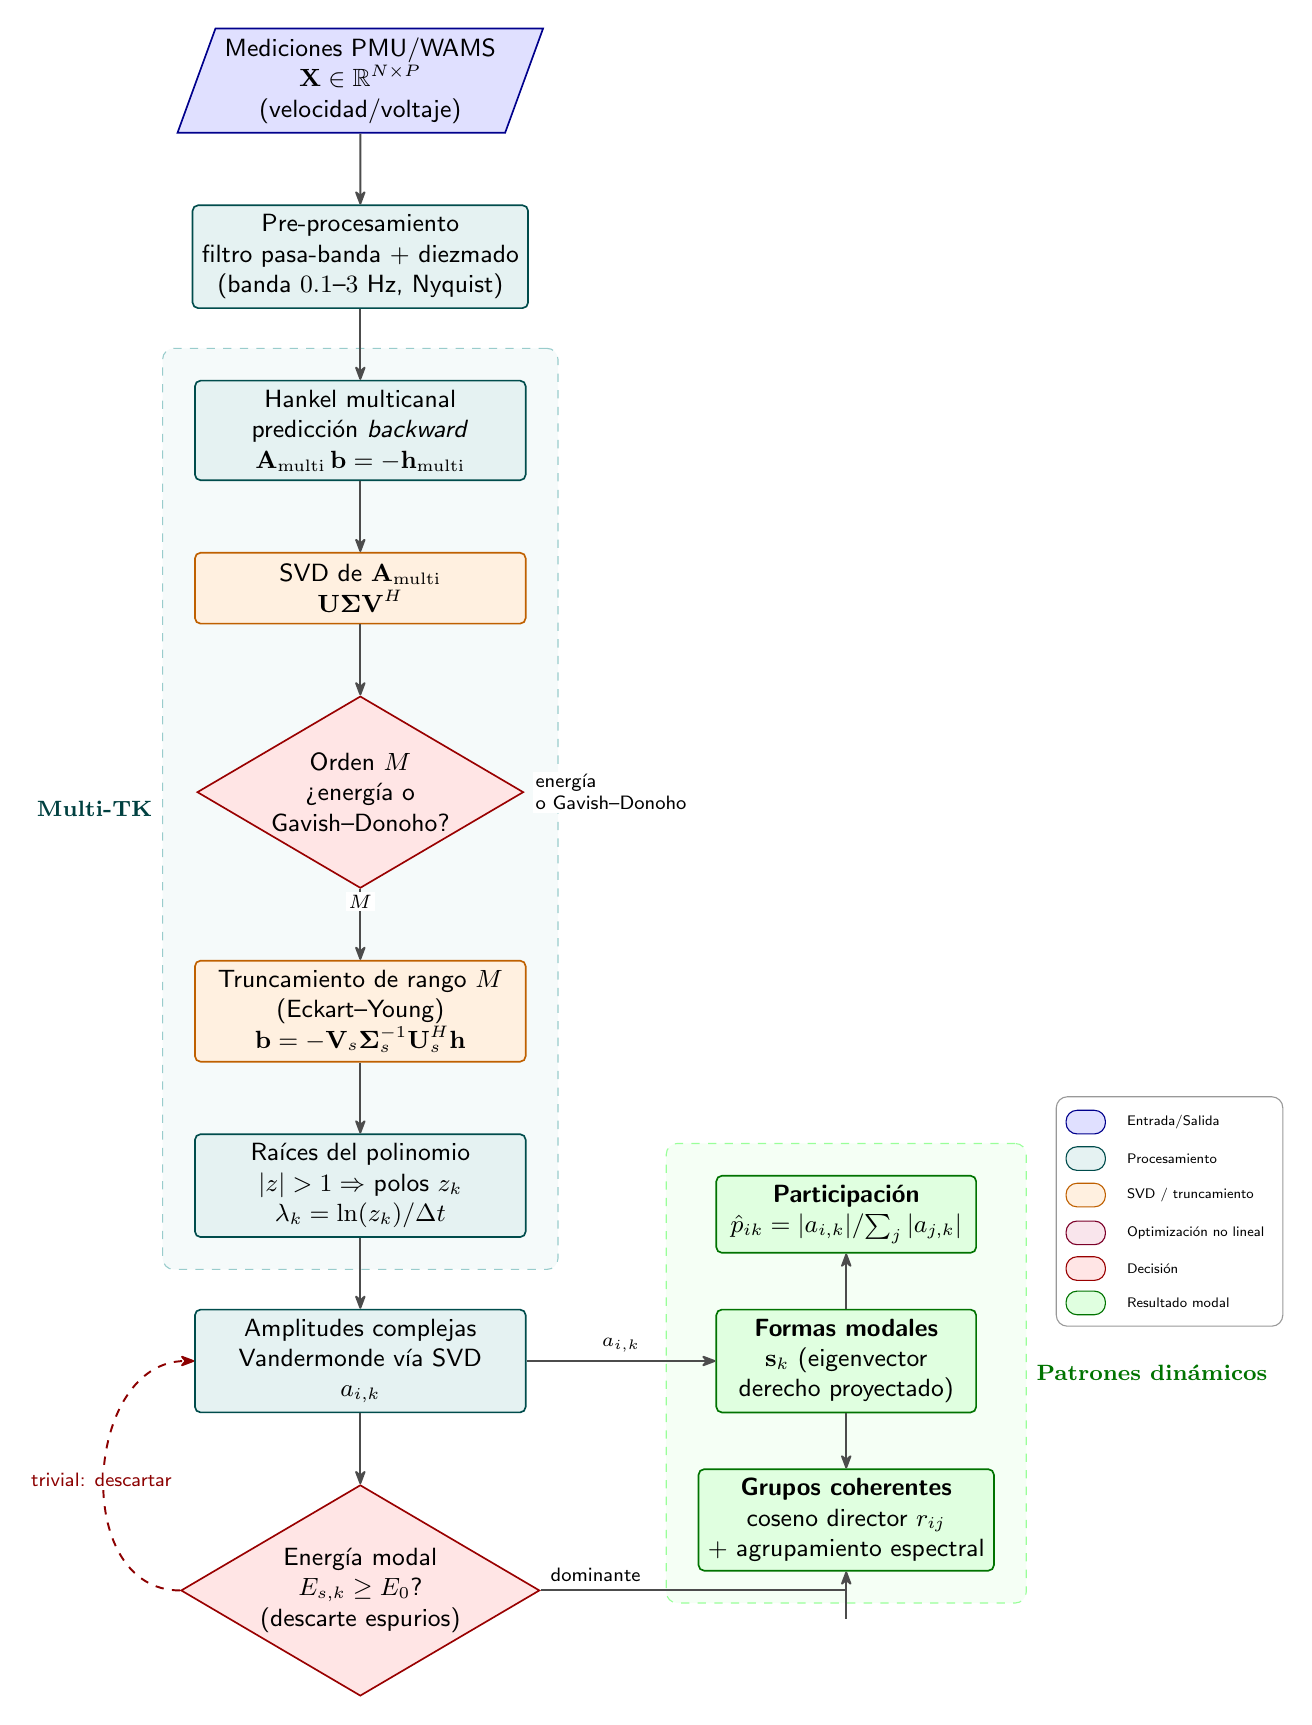
\begin{tikzpicture}[
    font=\small\sffamily,
    >={Stealth[round]},
    node distance = 9mm and 14mm,
    % --- estilos de caja ---
    io/.style    = {trapezium, trapezium left angle=70, trapezium right angle=110,
                    minimum width=30mm, minimum height=9mm, align=center,
                    draw=blue!55!black, fill=blue!12, line width=0.6pt},
    proc/.style  = {rectangle, rounded corners=2pt, minimum width=42mm,
                    minimum height=9mm, align=center,
                    draw=teal!60!black, fill=teal!10, line width=0.6pt},
    svd/.style   = {rectangle, rounded corners=2pt, minimum width=42mm,
                    minimum height=9mm, align=center,
                    draw=orange!75!black, fill=orange!12, line width=0.6pt},
    opt/.style   = {rectangle, rounded corners=2pt, minimum width=42mm,
                    minimum height=9mm, align=center,
                    draw=purple!65!black, fill=purple!10, line width=0.6pt},
    dec/.style   = {diamond, aspect=1.7, minimum width=30mm, align=center,
                    draw=red!60!black, fill=red!10, line width=0.6pt, inner sep=1pt},
    res/.style   = {rectangle, rounded corners=2pt, minimum width=33mm,
                    minimum height=9mm, align=center,
                    draw=green!45!black, fill=green!12, line width=0.6pt},
    arr/.style   = {->, line width=0.7pt, draw=black!70},
    lbl/.style   = {font=\scriptsize\sffamily, fill=white, inner sep=1pt}
]

% ===================== COLUMNA PRINCIPAL =====================
\node[io]   (data)  {Mediciones PMU/WAMS\\ $\mathbf{X}\in\mathbb{R}^{N\times P}$\\ (velocidad/voltaje)};
\node[proc] (pre)   [below=of data] {Pre-procesamiento\\ filtro pasa-banda $+$ diezmado\\ (banda $0.1$--$3$~Hz, Nyquist)};
\node[proc] (hank)  [below=of pre]  {Hankel multicanal\\ predicción \emph{backward}\\ $\mathbf{A}_{\mathrm{multi}}\,\mathbf{b}=-\mathbf{h}_{\mathrm{multi}}$};
\node[svd]  (svd)   [below=of hank] {SVD de $\mathbf{A}_{\mathrm{multi}}$\\ $\mathbf{U}\boldsymbol{\Sigma}\mathbf{V}^{H}$};
\node[dec]  (orden) [below=of svd]  {Orden $M$\\ ¿energía o\\ Gavish--Donoho?};
\node[svd]  (trunc) [below=of orden]{Truncamiento de rango $M$\\ (Eckart--Young)\\ $\mathbf{b}=-\mathbf{V}_s\boldsymbol{\Sigma}_s^{-1}\mathbf{U}_s^{H}\mathbf{h}$};
\node[proc] (roots) [below=of trunc]{Raíces del polinomio\\ $|z|>1 \Rightarrow$ polos $z_k$\\ $\lambda_k=\ln(z_k)/\Delta t$};
% --- Nodo OptVarPro ELIMINADO ---
\node[proc] (amp)   [below=of roots]{Amplitudes complejas\\ Vandermonde vía SVD\\ $a_{i,k}$};  % ahora debajo de roots
\node[dec]  (ener)  [below=of amp]  {Energía modal\\ $E_{s,k}\ge E_0$?\\ (descarte espurios)};

% ===================== RAMA DE PATRONES (derecha) =====================
\node[res] (shape) [right=24mm of amp]    {\textbf{Formas modales}\\ $\mathbf{s}_k$ (eigenvector\\ derecho proyectado)};
\node[res] (part)  [above=7mm of shape]   {\textbf{Participación}\\ $\hat p_{ik}=|a_{i,k}|/\!\sum_j|a_{j,k}|$};
\node[res] (coh)   [below=7mm of shape]   {\textbf{Grupos coherentes}\\ coseno director $r_{ij}$\\ $+$ agrupamiento espectral};

% ===================== FLECHAS PRINCIPALES =====================
\draw[arr] (data)  -- (pre);
\draw[arr] (pre)   -- (hank);
\draw[arr] (hank)  -- (svd);
\draw[arr] (svd)   -- (orden);
\draw[arr] (orden) -- (trunc);
\draw[arr] (trunc) -- (roots);
% Flecha directa de roots a amp (antes pasaba por varpro)
\draw[arr] (roots) -- (amp);
\draw[arr] (amp)   -- (ener);

% Etiqueta del orden M sobre la flecha orden->trunc
\node[lbl] at ($(orden)!0.5!(trunc)$) {$M$};

% Criterios de selección de orden
\node[lbl, right=1mm of orden, align=left] {energ\'ia\\ o Gavish--Donoho};

% Energía modal: si pasa (dominante) alimenta los patrones
\draw[arr] (ener.east) -| ($(coh.south)+(0,-6mm)$) -- (coh.south);
\node[lbl] at ($(ener.east)+(7mm,2mm)$) {dominante};

% Amplitudes -> formas modales
\draw[arr] (amp.east) -- (shape.west);
\node[lbl] at ($(amp.east)!0.5!(shape.west)+(0,2mm)$) {$a_{i,k}$};

\draw[arr] (shape.north) -- (part.south);
\draw[arr] (shape.south) -- (coh.north);

% Retro de descarte (modo trivial vuelve, lazo corto a la izquierda)
\draw[arr, dashed, draw=red!55!black]
    (ener.west) .. controls +(-1.4,0) and +(-1.4,0) .. (amp.west);
\node[lbl, text=red!55!black] at ($(ener.west)+(-1.0,1.4)$) {trivial: descartar};

% ===================== FONDOS POR ETAPA =====================
\begin{scope}[on background layer]
    \node[draw=teal!40, dashed, rounded corners, fill=teal!4, inner sep=4mm,
          fit=(hank)(roots), label={[teal!50!black,font=\footnotesize\bfseries]left:Multi-TK}] {};
    % --- CAJA OptVarPro ELIMINADA ---
    \node[draw=green!40, dashed, rounded corners, fill=green!4, inner sep=4mm,
          fit=(part)(shape)(coh),
          label={[green!45!black,font=\footnotesize\bfseries]right:Patrones dinámicos}] {};
\end{scope}

% ===================== LEYENDA =====================
\matrix [draw=black!40, rounded corners, fill=white, anchor=north west,
         column sep=1.5mm, row sep=0.8mm, font=\tiny\sffamily,
         every node/.style={anchor=west}]
    at ($(part.north east)+(10mm,10mm)$) {
    \node[draw=blue!55!black,   fill=blue!12,   minimum width=5mm, minimum height=3mm]{}; & \node{Entrada/Salida}; \\
    \node[draw=teal!60!black,   fill=teal!10,   minimum width=5mm, minimum height=3mm]{}; & \node{Procesamiento}; \\
    \node[draw=orange!75!black, fill=orange!12, minimum width=5mm, minimum height=3mm]{}; & \node{SVD / truncamiento}; \\
    \node[draw=purple!65!black, fill=purple!10, minimum width=5mm, minimum height=3mm]{}; & \node{Optimizaci\'on no lineal}; \\
    \node[draw=red!60!black,    fill=red!10,    minimum width=5mm, minimum height=3mm]{}; & \node{Decisi\'on}; \\
    \node[draw=green!45!black,  fill=green!12,  minimum width=5mm, minimum height=3mm]{}; & \node{Resultado modal}; \\
};

\end{tikzpicture}
\endgroup

% ---------- cierre del bloque standalone (descomentar si se activa arriba) ----------
\end{document}}
%     \caption[...]{...}
%     \label{fig:metodologia}
%   \end{figure}
%   NO compiles este archivo por separado (a menos que descomentes el bloque standalone).
%
% PAQUETES requeridos en el preámbulo de la tesis (¡imprescindibles!)

% ---------- BLOQUE STANDALONE (comentado; descomentar solo para prueba) ----------
 \documentclass[border=6pt]{standalone}
 \usepackage[utf8]{inputenc}
 \usepackage[T1]{fontenc}
 \usepackage{amsmath}
\usepackage{amssymb}
 \usepackage{tikz} \usetikzlibrary{shapes.geometric, arrows.meta, positioning, calc, fit, backgrounds}
 \begin{document}
% ------------------------------------------------------------------------

% Protección para babel español: desactiva localmente los shorthands < y >
% que interfieren con las puntas de flecha de TikZ (>={Stealth}, ->, -|).
\begingroup
\ifcsname shorthandoff\endcsname
  \shorthandoff{<>}
\fi
%
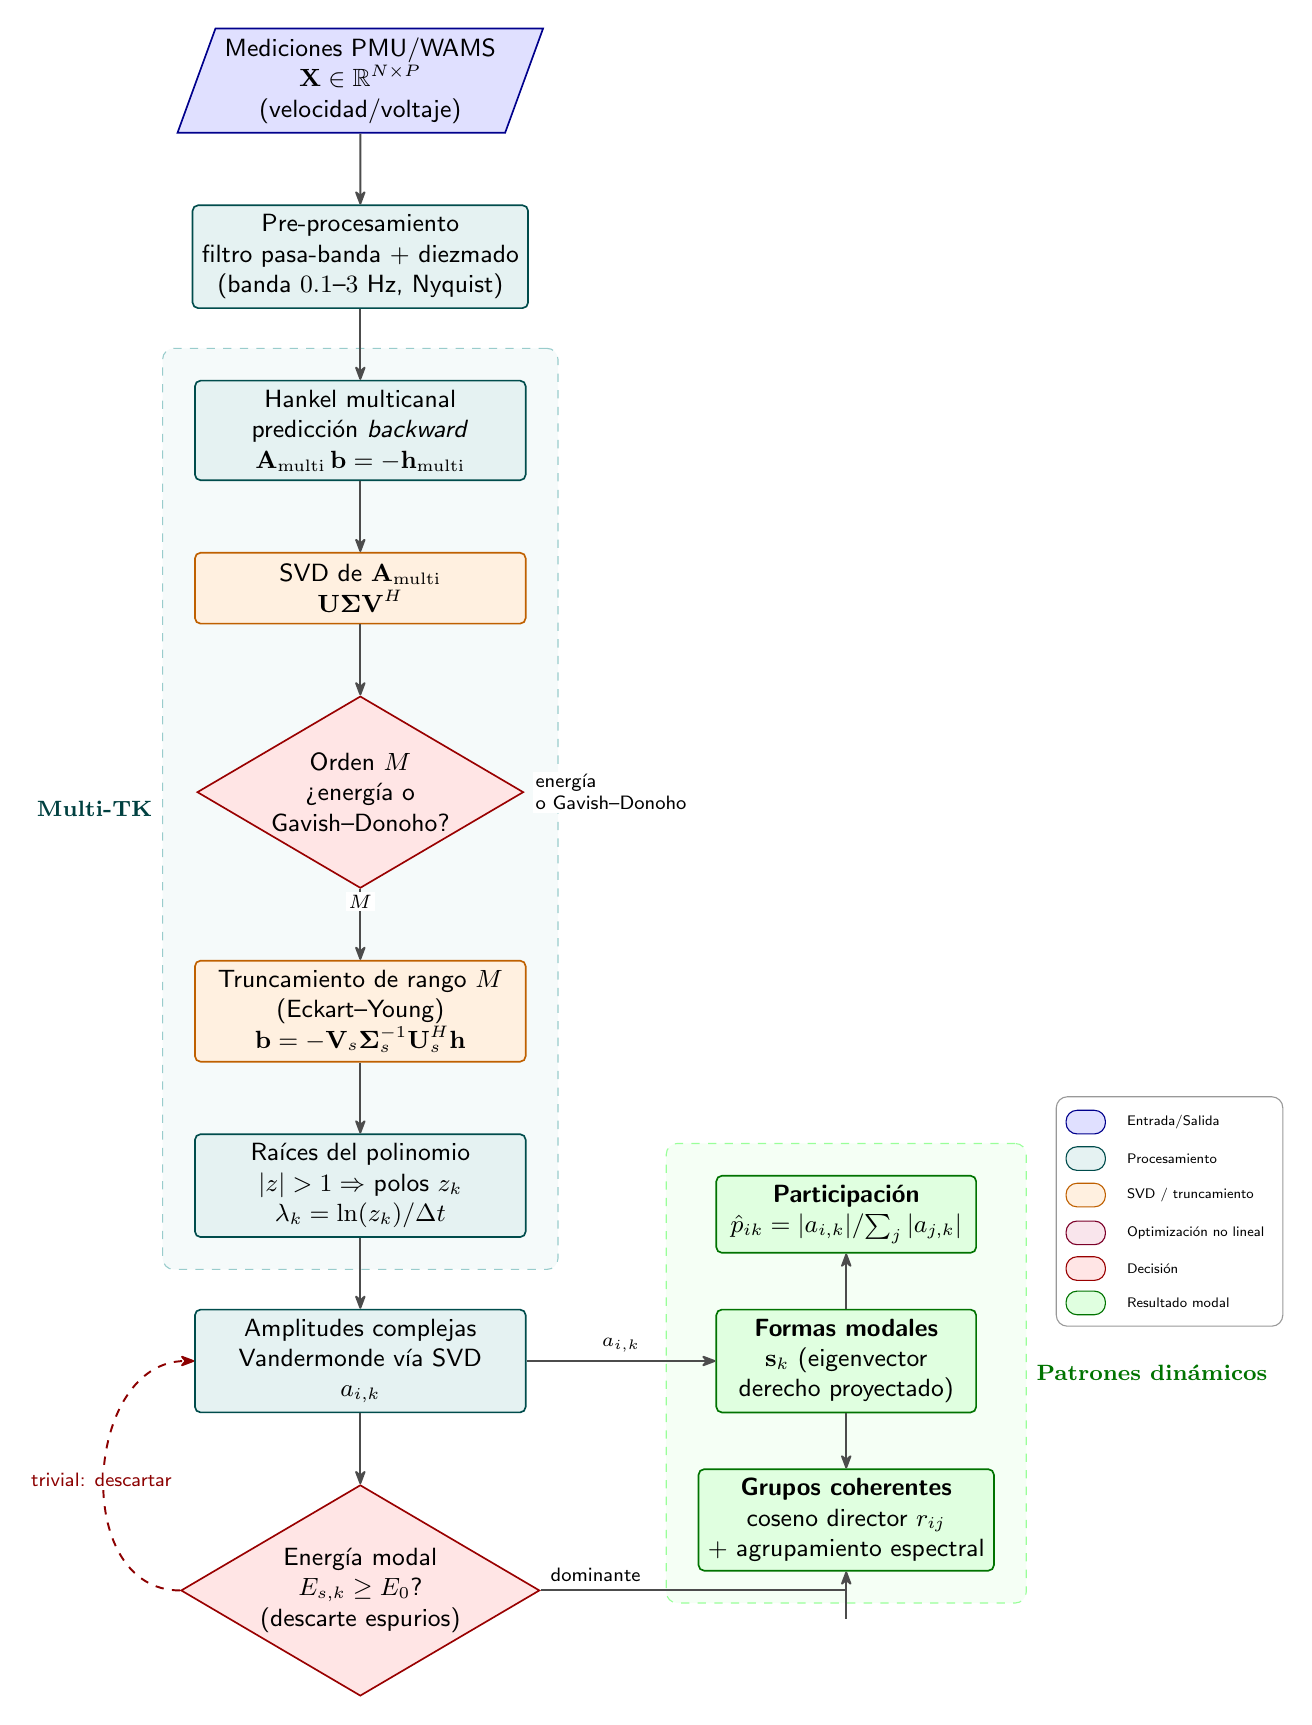
\begin{tikzpicture}[
    font=\small\sffamily,
    >={Stealth[round]},
    node distance = 9mm and 14mm,
    % --- estilos de caja ---
    io/.style    = {trapezium, trapezium left angle=70, trapezium right angle=110,
                    minimum width=30mm, minimum height=9mm, align=center,
                    draw=blue!55!black, fill=blue!12, line width=0.6pt},
    proc/.style  = {rectangle, rounded corners=2pt, minimum width=42mm,
                    minimum height=9mm, align=center,
                    draw=teal!60!black, fill=teal!10, line width=0.6pt},
    svd/.style   = {rectangle, rounded corners=2pt, minimum width=42mm,
                    minimum height=9mm, align=center,
                    draw=orange!75!black, fill=orange!12, line width=0.6pt},
    opt/.style   = {rectangle, rounded corners=2pt, minimum width=42mm,
                    minimum height=9mm, align=center,
                    draw=purple!65!black, fill=purple!10, line width=0.6pt},
    dec/.style   = {diamond, aspect=1.7, minimum width=30mm, align=center,
                    draw=red!60!black, fill=red!10, line width=0.6pt, inner sep=1pt},
    res/.style   = {rectangle, rounded corners=2pt, minimum width=33mm,
                    minimum height=9mm, align=center,
                    draw=green!45!black, fill=green!12, line width=0.6pt},
    arr/.style   = {->, line width=0.7pt, draw=black!70},
    lbl/.style   = {font=\scriptsize\sffamily, fill=white, inner sep=1pt}
]

% ===================== COLUMNA PRINCIPAL =====================
\node[io]   (data)  {Mediciones PMU/WAMS\\ $\mathbf{X}\in\mathbb{R}^{N\times P}$\\ (velocidad/voltaje)};
\node[proc] (pre)   [below=of data] {Pre-procesamiento\\ filtro pasa-banda $+$ diezmado\\ (banda $0.1$--$3$~Hz, Nyquist)};
\node[proc] (hank)  [below=of pre]  {Hankel multicanal\\ predicción \emph{backward}\\ $\mathbf{A}_{\mathrm{multi}}\,\mathbf{b}=-\mathbf{h}_{\mathrm{multi}}$};
\node[svd]  (svd)   [below=of hank] {SVD de $\mathbf{A}_{\mathrm{multi}}$\\ $\mathbf{U}\boldsymbol{\Sigma}\mathbf{V}^{H}$};
\node[dec]  (orden) [below=of svd]  {Orden $M$\\ ¿energía o\\ Gavish--Donoho?};
\node[svd]  (trunc) [below=of orden]{Truncamiento de rango $M$\\ (Eckart--Young)\\ $\mathbf{b}=-\mathbf{V}_s\boldsymbol{\Sigma}_s^{-1}\mathbf{U}_s^{H}\mathbf{h}$};
\node[proc] (roots) [below=of trunc]{Raíces del polinomio\\ $|z|>1 \Rightarrow$ polos $z_k$\\ $\lambda_k=\ln(z_k)/\Delta t$};
% --- Nodo OptVarPro ELIMINADO ---
\node[proc] (amp)   [below=of roots]{Amplitudes complejas\\ Vandermonde vía SVD\\ $a_{i,k}$};  % ahora debajo de roots
\node[dec]  (ener)  [below=of amp]  {Energía modal\\ $E_{s,k}\ge E_0$?\\ (descarte espurios)};

% ===================== RAMA DE PATRONES (derecha) =====================
\node[res] (shape) [right=24mm of amp]    {\textbf{Formas modales}\\ $\mathbf{s}_k$ (eigenvector\\ derecho proyectado)};
\node[res] (part)  [above=7mm of shape]   {\textbf{Participación}\\ $\hat p_{ik}=|a_{i,k}|/\!\sum_j|a_{j,k}|$};
\node[res] (coh)   [below=7mm of shape]   {\textbf{Grupos coherentes}\\ coseno director $r_{ij}$\\ $+$ agrupamiento espectral};

% ===================== FLECHAS PRINCIPALES =====================
\draw[arr] (data)  -- (pre);
\draw[arr] (pre)   -- (hank);
\draw[arr] (hank)  -- (svd);
\draw[arr] (svd)   -- (orden);
\draw[arr] (orden) -- (trunc);
\draw[arr] (trunc) -- (roots);
% Flecha directa de roots a amp (antes pasaba por varpro)
\draw[arr] (roots) -- (amp);
\draw[arr] (amp)   -- (ener);

% Etiqueta del orden M sobre la flecha orden->trunc
\node[lbl] at ($(orden)!0.5!(trunc)$) {$M$};

% Criterios de selección de orden
\node[lbl, right=1mm of orden, align=left] {energ\'ia\\ o Gavish--Donoho};

% Energía modal: si pasa (dominante) alimenta los patrones
\draw[arr] (ener.east) -| ($(coh.south)+(0,-6mm)$) -- (coh.south);
\node[lbl] at ($(ener.east)+(7mm,2mm)$) {dominante};

% Amplitudes -> formas modales
\draw[arr] (amp.east) -- (shape.west);
\node[lbl] at ($(amp.east)!0.5!(shape.west)+(0,2mm)$) {$a_{i,k}$};

\draw[arr] (shape.north) -- (part.south);
\draw[arr] (shape.south) -- (coh.north);

% Retro de descarte (modo trivial vuelve, lazo corto a la izquierda)
\draw[arr, dashed, draw=red!55!black]
    (ener.west) .. controls +(-1.4,0) and +(-1.4,0) .. (amp.west);
\node[lbl, text=red!55!black] at ($(ener.west)+(-1.0,1.4)$) {trivial: descartar};

% ===================== FONDOS POR ETAPA =====================
\begin{scope}[on background layer]
    \node[draw=teal!40, dashed, rounded corners, fill=teal!4, inner sep=4mm,
          fit=(hank)(roots), label={[teal!50!black,font=\footnotesize\bfseries]left:Multi-TK}] {};
    % --- CAJA OptVarPro ELIMINADA ---
    \node[draw=green!40, dashed, rounded corners, fill=green!4, inner sep=4mm,
          fit=(part)(shape)(coh),
          label={[green!45!black,font=\footnotesize\bfseries]right:Patrones dinámicos}] {};
\end{scope}

% ===================== LEYENDA =====================
\matrix [draw=black!40, rounded corners, fill=white, anchor=north west,
         column sep=1.5mm, row sep=0.8mm, font=\tiny\sffamily,
         every node/.style={anchor=west}]
    at ($(part.north east)+(10mm,10mm)$) {
    \node[draw=blue!55!black,   fill=blue!12,   minimum width=5mm, minimum height=3mm]{}; & \node{Entrada/Salida}; \\
    \node[draw=teal!60!black,   fill=teal!10,   minimum width=5mm, minimum height=3mm]{}; & \node{Procesamiento}; \\
    \node[draw=orange!75!black, fill=orange!12, minimum width=5mm, minimum height=3mm]{}; & \node{SVD / truncamiento}; \\
    \node[draw=purple!65!black, fill=purple!10, minimum width=5mm, minimum height=3mm]{}; & \node{Optimizaci\'on no lineal}; \\
    \node[draw=red!60!black,    fill=red!10,    minimum width=5mm, minimum height=3mm]{}; & \node{Decisi\'on}; \\
    \node[draw=green!45!black,  fill=green!12,  minimum width=5mm, minimum height=3mm]{}; & \node{Resultado modal}; \\
};

\end{tikzpicture}
\endgroup

% ---------- cierre del bloque standalone (descomentar si se activa arriba) ----------
\end{document}}
%     \caption[...]{...}
%     \label{fig:metodologia}
%   \end{figure}
%   NO compiles este archivo por separado (a menos que descomentes el bloque standalone).
%
% PAQUETES requeridos en el preámbulo de la tesis (¡imprescindibles!)

% ---------- BLOQUE STANDALONE (comentado; descomentar solo para prueba) ----------
 \documentclass[border=6pt]{standalone}
 \usepackage[utf8]{inputenc}
 \usepackage[T1]{fontenc}
 \usepackage{amsmath}
\usepackage{amssymb}
 \usepackage{tikz} \usetikzlibrary{shapes.geometric, arrows.meta, positioning, calc, fit, backgrounds}
 \begin{document}
% ------------------------------------------------------------------------

% Protección para babel español: desactiva localmente los shorthands < y >
% que interfieren con las puntas de flecha de TikZ (>={Stealth}, ->, -|).
\begingroup
\ifcsname shorthandoff\endcsname
  \shorthandoff{<>}
\fi
%
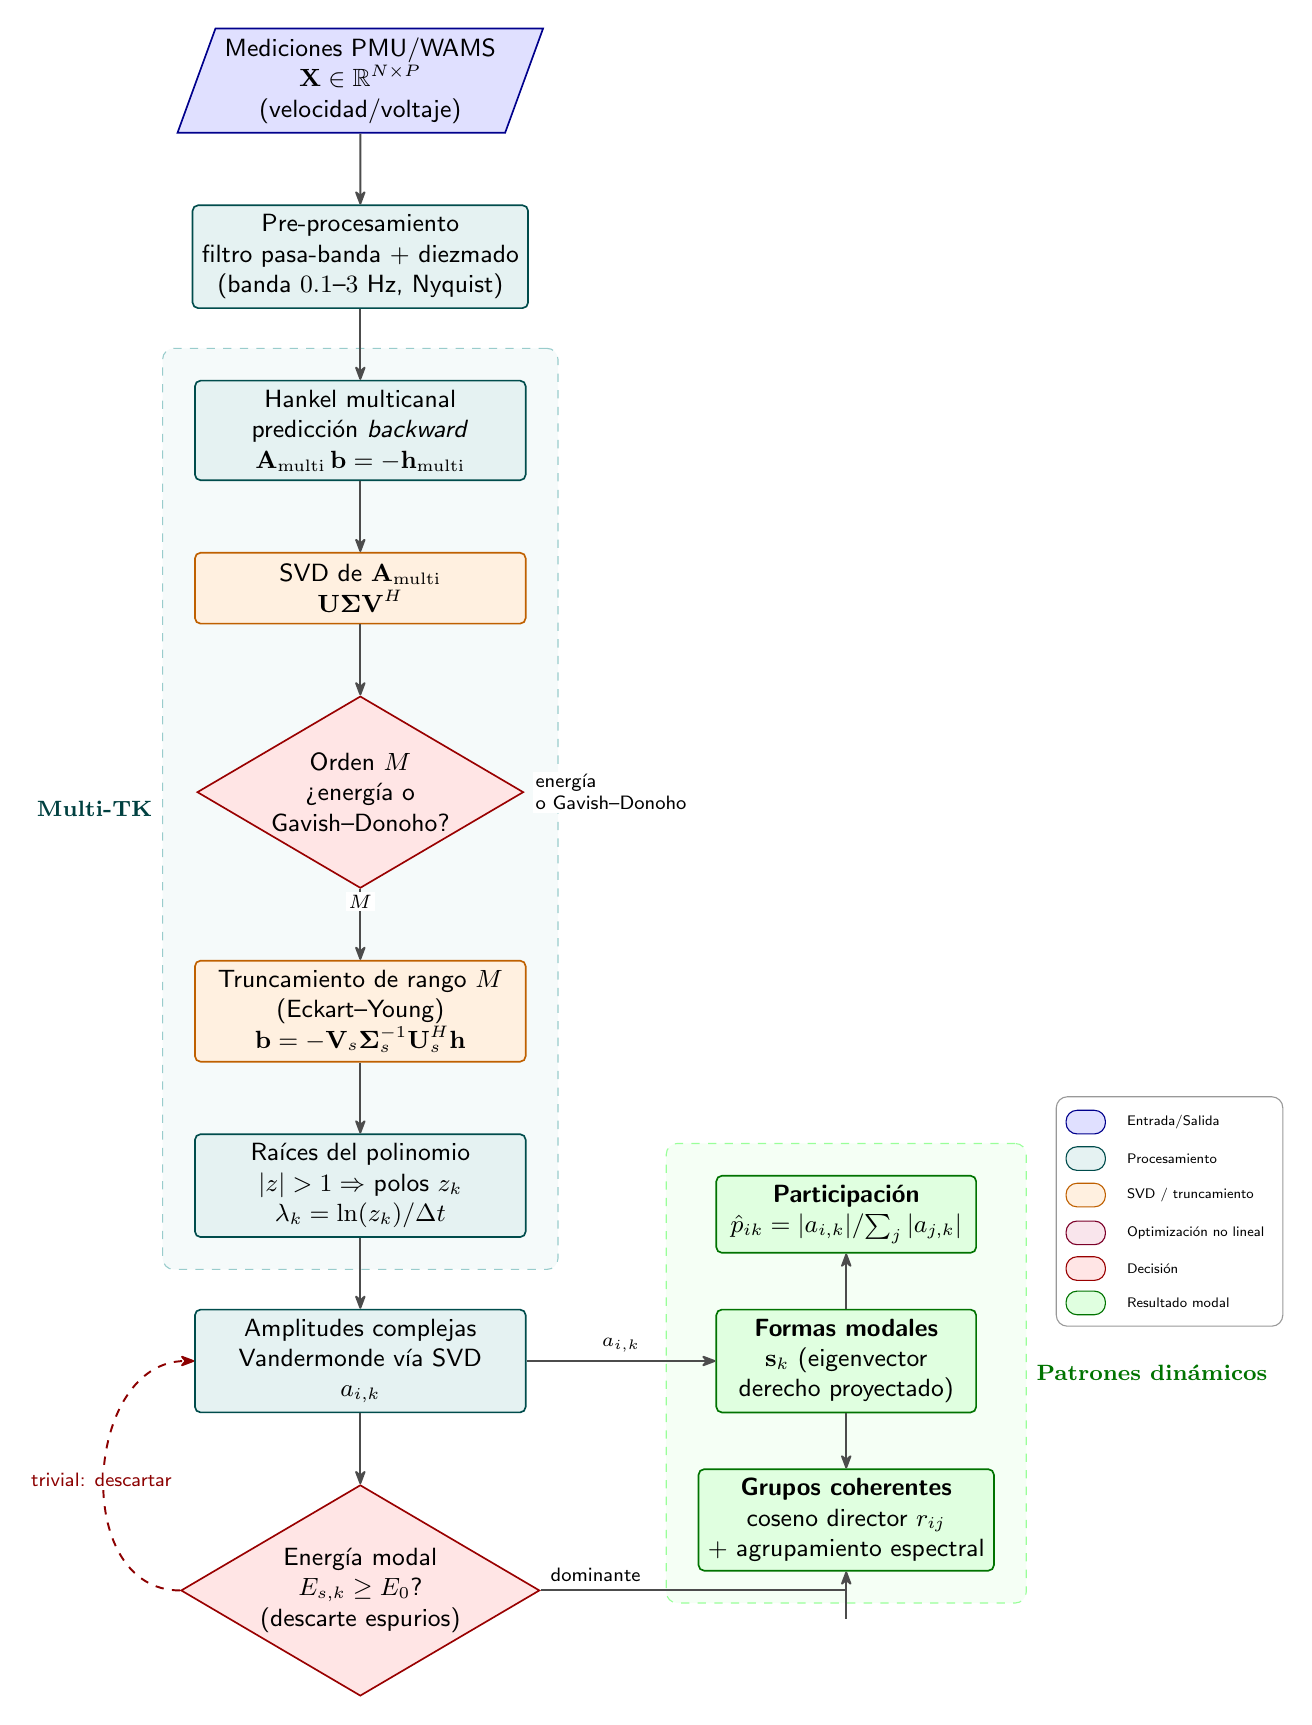
\begin{tikzpicture}[
    font=\small\sffamily,
    >={Stealth[round]},
    node distance = 9mm and 14mm,
    % --- estilos de caja ---
    io/.style    = {trapezium, trapezium left angle=70, trapezium right angle=110,
                    minimum width=30mm, minimum height=9mm, align=center,
                    draw=blue!55!black, fill=blue!12, line width=0.6pt},
    proc/.style  = {rectangle, rounded corners=2pt, minimum width=42mm,
                    minimum height=9mm, align=center,
                    draw=teal!60!black, fill=teal!10, line width=0.6pt},
    svd/.style   = {rectangle, rounded corners=2pt, minimum width=42mm,
                    minimum height=9mm, align=center,
                    draw=orange!75!black, fill=orange!12, line width=0.6pt},
    opt/.style   = {rectangle, rounded corners=2pt, minimum width=42mm,
                    minimum height=9mm, align=center,
                    draw=purple!65!black, fill=purple!10, line width=0.6pt},
    dec/.style   = {diamond, aspect=1.7, minimum width=30mm, align=center,
                    draw=red!60!black, fill=red!10, line width=0.6pt, inner sep=1pt},
    res/.style   = {rectangle, rounded corners=2pt, minimum width=33mm,
                    minimum height=9mm, align=center,
                    draw=green!45!black, fill=green!12, line width=0.6pt},
    arr/.style   = {->, line width=0.7pt, draw=black!70},
    lbl/.style   = {font=\scriptsize\sffamily, fill=white, inner sep=1pt}
]

% ===================== COLUMNA PRINCIPAL =====================
\node[io]   (data)  {Mediciones PMU/WAMS\\ $\mathbf{X}\in\mathbb{R}^{N\times P}$\\ (velocidad/voltaje)};
\node[proc] (pre)   [below=of data] {Pre-procesamiento\\ filtro pasa-banda $+$ diezmado\\ (banda $0.1$--$3$~Hz, Nyquist)};
\node[proc] (hank)  [below=of pre]  {Hankel multicanal\\ predicción \emph{backward}\\ $\mathbf{A}_{\mathrm{multi}}\,\mathbf{b}=-\mathbf{h}_{\mathrm{multi}}$};
\node[svd]  (svd)   [below=of hank] {SVD de $\mathbf{A}_{\mathrm{multi}}$\\ $\mathbf{U}\boldsymbol{\Sigma}\mathbf{V}^{H}$};
\node[dec]  (orden) [below=of svd]  {Orden $M$\\ ¿energía o\\ Gavish--Donoho?};
\node[svd]  (trunc) [below=of orden]{Truncamiento de rango $M$\\ (Eckart--Young)\\ $\mathbf{b}=-\mathbf{V}_s\boldsymbol{\Sigma}_s^{-1}\mathbf{U}_s^{H}\mathbf{h}$};
\node[proc] (roots) [below=of trunc]{Raíces del polinomio\\ $|z|>1 \Rightarrow$ polos $z_k$\\ $\lambda_k=\ln(z_k)/\Delta t$};
% --- Nodo OptVarPro ELIMINADO ---
\node[proc] (amp)   [below=of roots]{Amplitudes complejas\\ Vandermonde vía SVD\\ $a_{i,k}$};  % ahora debajo de roots
\node[dec]  (ener)  [below=of amp]  {Energía modal\\ $E_{s,k}\ge E_0$?\\ (descarte espurios)};

% ===================== RAMA DE PATRONES (derecha) =====================
\node[res] (shape) [right=24mm of amp]    {\textbf{Formas modales}\\ $\mathbf{s}_k$ (eigenvector\\ derecho proyectado)};
\node[res] (part)  [above=7mm of shape]   {\textbf{Participación}\\ $\hat p_{ik}=|a_{i,k}|/\!\sum_j|a_{j,k}|$};
\node[res] (coh)   [below=7mm of shape]   {\textbf{Grupos coherentes}\\ coseno director $r_{ij}$\\ $+$ agrupamiento espectral};

% ===================== FLECHAS PRINCIPALES =====================
\draw[arr] (data)  -- (pre);
\draw[arr] (pre)   -- (hank);
\draw[arr] (hank)  -- (svd);
\draw[arr] (svd)   -- (orden);
\draw[arr] (orden) -- (trunc);
\draw[arr] (trunc) -- (roots);
% Flecha directa de roots a amp (antes pasaba por varpro)
\draw[arr] (roots) -- (amp);
\draw[arr] (amp)   -- (ener);

% Etiqueta del orden M sobre la flecha orden->trunc
\node[lbl] at ($(orden)!0.5!(trunc)$) {$M$};

% Criterios de selección de orden
\node[lbl, right=1mm of orden, align=left] {energ\'ia\\ o Gavish--Donoho};

% Energía modal: si pasa (dominante) alimenta los patrones
\draw[arr] (ener.east) -| ($(coh.south)+(0,-6mm)$) -- (coh.south);
\node[lbl] at ($(ener.east)+(7mm,2mm)$) {dominante};

% Amplitudes -> formas modales
\draw[arr] (amp.east) -- (shape.west);
\node[lbl] at ($(amp.east)!0.5!(shape.west)+(0,2mm)$) {$a_{i,k}$};

\draw[arr] (shape.north) -- (part.south);
\draw[arr] (shape.south) -- (coh.north);

% Retro de descarte (modo trivial vuelve, lazo corto a la izquierda)
\draw[arr, dashed, draw=red!55!black]
    (ener.west) .. controls +(-1.4,0) and +(-1.4,0) .. (amp.west);
\node[lbl, text=red!55!black] at ($(ener.west)+(-1.0,1.4)$) {trivial: descartar};

% ===================== FONDOS POR ETAPA =====================
\begin{scope}[on background layer]
    \node[draw=teal!40, dashed, rounded corners, fill=teal!4, inner sep=4mm,
          fit=(hank)(roots), label={[teal!50!black,font=\footnotesize\bfseries]left:Multi-TK}] {};
    % --- CAJA OptVarPro ELIMINADA ---
    \node[draw=green!40, dashed, rounded corners, fill=green!4, inner sep=4mm,
          fit=(part)(shape)(coh),
          label={[green!45!black,font=\footnotesize\bfseries]right:Patrones dinámicos}] {};
\end{scope}

% ===================== LEYENDA =====================
\matrix [draw=black!40, rounded corners, fill=white, anchor=north west,
         column sep=1.5mm, row sep=0.8mm, font=\tiny\sffamily,
         every node/.style={anchor=west}]
    at ($(part.north east)+(10mm,10mm)$) {
    \node[draw=blue!55!black,   fill=blue!12,   minimum width=5mm, minimum height=3mm]{}; & \node{Entrada/Salida}; \\
    \node[draw=teal!60!black,   fill=teal!10,   minimum width=5mm, minimum height=3mm]{}; & \node{Procesamiento}; \\
    \node[draw=orange!75!black, fill=orange!12, minimum width=5mm, minimum height=3mm]{}; & \node{SVD / truncamiento}; \\
    \node[draw=purple!65!black, fill=purple!10, minimum width=5mm, minimum height=3mm]{}; & \node{Optimizaci\'on no lineal}; \\
    \node[draw=red!60!black,    fill=red!10,    minimum width=5mm, minimum height=3mm]{}; & \node{Decisi\'on}; \\
    \node[draw=green!45!black,  fill=green!12,  minimum width=5mm, minimum height=3mm]{}; & \node{Resultado modal}; \\
};

\end{tikzpicture}
\endgroup

% ---------- cierre del bloque standalone (descomentar si se activa arriba) ----------
\end{document}}
%     \caption[...]{...}
%     \label{fig:metodologia}
%   \end{figure}
%   NO compiles este archivo por separado (a menos que descomentes el bloque standalone).
%
% PAQUETES requeridos en el preámbulo de la tesis (¡imprescindibles!)

% ---------- BLOQUE STANDALONE (comentado; descomentar solo para prueba) ----------
 \documentclass[border=6pt]{standalone}
 \usepackage[utf8]{inputenc}
 \usepackage[T1]{fontenc}
 \usepackage{amsmath}
\usepackage{amssymb}
 \usepackage{tikz} \usetikzlibrary{shapes.geometric, arrows.meta, positioning, calc, fit, backgrounds}
 \begin{document}
% ------------------------------------------------------------------------

% Protección para babel español: desactiva localmente los shorthands < y >
% que interfieren con las puntas de flecha de TikZ (>={Stealth}, ->, -|).
\begingroup
\ifcsname shorthandoff\endcsname
  \shorthandoff{<>}
\fi
%
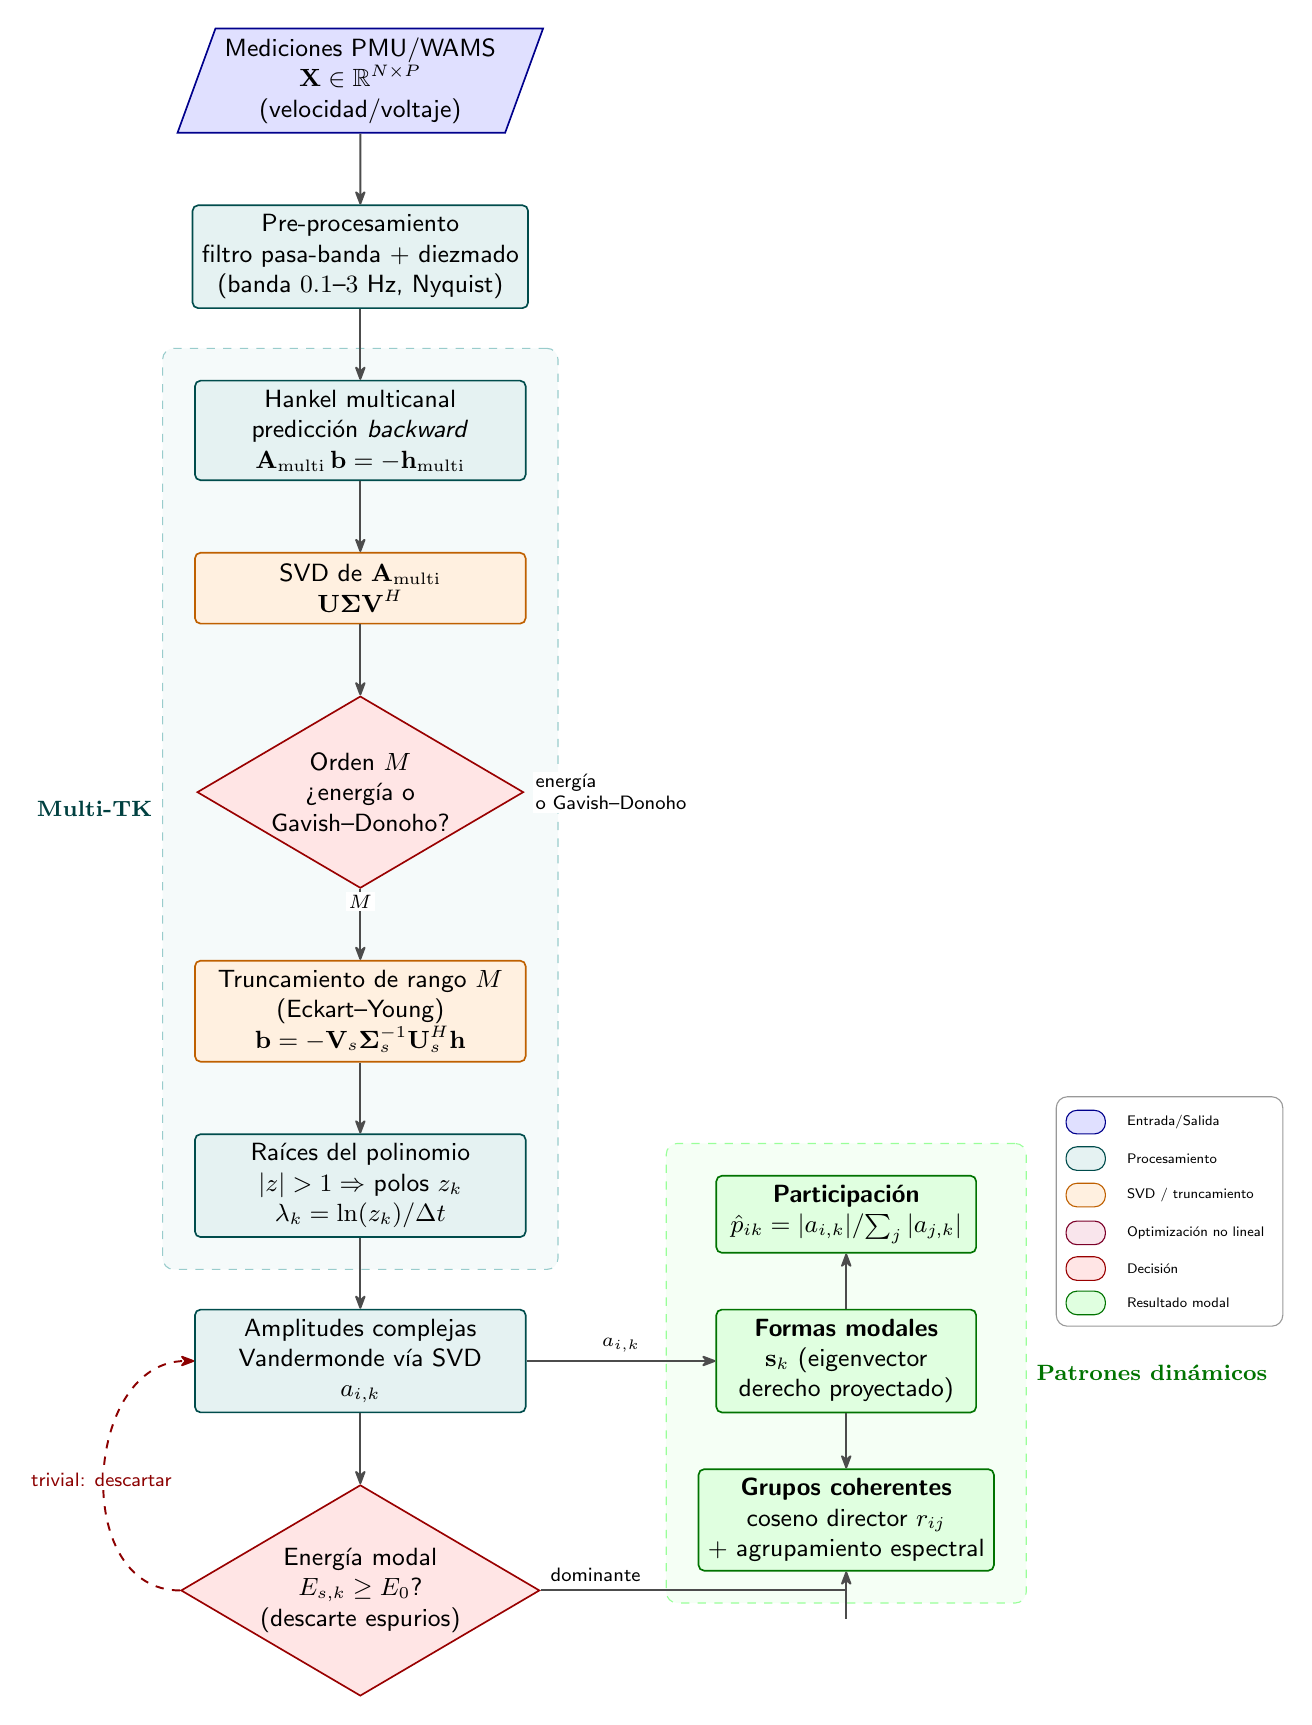
\begin{tikzpicture}[
    font=\small\sffamily,
    >={Stealth[round]},
    node distance = 9mm and 14mm,
    % --- estilos de caja ---
    io/.style    = {trapezium, trapezium left angle=70, trapezium right angle=110,
                    minimum width=30mm, minimum height=9mm, align=center,
                    draw=blue!55!black, fill=blue!12, line width=0.6pt},
    proc/.style  = {rectangle, rounded corners=2pt, minimum width=42mm,
                    minimum height=9mm, align=center,
                    draw=teal!60!black, fill=teal!10, line width=0.6pt},
    svd/.style   = {rectangle, rounded corners=2pt, minimum width=42mm,
                    minimum height=9mm, align=center,
                    draw=orange!75!black, fill=orange!12, line width=0.6pt},
    opt/.style   = {rectangle, rounded corners=2pt, minimum width=42mm,
                    minimum height=9mm, align=center,
                    draw=purple!65!black, fill=purple!10, line width=0.6pt},
    dec/.style   = {diamond, aspect=1.7, minimum width=30mm, align=center,
                    draw=red!60!black, fill=red!10, line width=0.6pt, inner sep=1pt},
    res/.style   = {rectangle, rounded corners=2pt, minimum width=33mm,
                    minimum height=9mm, align=center,
                    draw=green!45!black, fill=green!12, line width=0.6pt},
    arr/.style   = {->, line width=0.7pt, draw=black!70},
    lbl/.style   = {font=\scriptsize\sffamily, fill=white, inner sep=1pt}
]

% ===================== COLUMNA PRINCIPAL =====================
\node[io]   (data)  {Mediciones PMU/WAMS\\ $\mathbf{X}\in\mathbb{R}^{N\times P}$\\ (velocidad/voltaje)};
\node[proc] (pre)   [below=of data] {Pre-procesamiento\\ filtro pasa-banda $+$ diezmado\\ (banda $0.1$--$3$~Hz, Nyquist)};
\node[proc] (hank)  [below=of pre]  {Hankel multicanal\\ predicción \emph{backward}\\ $\mathbf{A}_{\mathrm{multi}}\,\mathbf{b}=-\mathbf{h}_{\mathrm{multi}}$};
\node[svd]  (svd)   [below=of hank] {SVD de $\mathbf{A}_{\mathrm{multi}}$\\ $\mathbf{U}\boldsymbol{\Sigma}\mathbf{V}^{H}$};
\node[dec]  (orden) [below=of svd]  {Orden $M$\\ ¿energía o\\ Gavish--Donoho?};
\node[svd]  (trunc) [below=of orden]{Truncamiento de rango $M$\\ (Eckart--Young)\\ $\mathbf{b}=-\mathbf{V}_s\boldsymbol{\Sigma}_s^{-1}\mathbf{U}_s^{H}\mathbf{h}$};
\node[proc] (roots) [below=of trunc]{Raíces del polinomio\\ $|z|>1 \Rightarrow$ polos $z_k$\\ $\lambda_k=\ln(z_k)/\Delta t$};
% --- Nodo OptVarPro ELIMINADO ---
\node[proc] (amp)   [below=of roots]{Amplitudes complejas\\ Vandermonde vía SVD\\ $a_{i,k}$};  % ahora debajo de roots
\node[dec]  (ener)  [below=of amp]  {Energía modal\\ $E_{s,k}\ge E_0$?\\ (descarte espurios)};

% ===================== RAMA DE PATRONES (derecha) =====================
\node[res] (shape) [right=24mm of amp]    {\textbf{Formas modales}\\ $\mathbf{s}_k$ (eigenvector\\ derecho proyectado)};
\node[res] (part)  [above=7mm of shape]   {\textbf{Participación}\\ $\hat p_{ik}=|a_{i,k}|/\!\sum_j|a_{j,k}|$};
\node[res] (coh)   [below=7mm of shape]   {\textbf{Grupos coherentes}\\ coseno director $r_{ij}$\\ $+$ agrupamiento espectral};

% ===================== FLECHAS PRINCIPALES =====================
\draw[arr] (data)  -- (pre);
\draw[arr] (pre)   -- (hank);
\draw[arr] (hank)  -- (svd);
\draw[arr] (svd)   -- (orden);
\draw[arr] (orden) -- (trunc);
\draw[arr] (trunc) -- (roots);
% Flecha directa de roots a amp (antes pasaba por varpro)
\draw[arr] (roots) -- (amp);
\draw[arr] (amp)   -- (ener);

% Etiqueta del orden M sobre la flecha orden->trunc
\node[lbl] at ($(orden)!0.5!(trunc)$) {$M$};

% Criterios de selección de orden
\node[lbl, right=1mm of orden, align=left] {energ\'ia\\ o Gavish--Donoho};

% Energía modal: si pasa (dominante) alimenta los patrones
\draw[arr] (ener.east) -| ($(coh.south)+(0,-6mm)$) -- (coh.south);
\node[lbl] at ($(ener.east)+(7mm,2mm)$) {dominante};

% Amplitudes -> formas modales
\draw[arr] (amp.east) -- (shape.west);
\node[lbl] at ($(amp.east)!0.5!(shape.west)+(0,2mm)$) {$a_{i,k}$};

\draw[arr] (shape.north) -- (part.south);
\draw[arr] (shape.south) -- (coh.north);

% Retro de descarte (modo trivial vuelve, lazo corto a la izquierda)
\draw[arr, dashed, draw=red!55!black]
    (ener.west) .. controls +(-1.4,0) and +(-1.4,0) .. (amp.west);
\node[lbl, text=red!55!black] at ($(ener.west)+(-1.0,1.4)$) {trivial: descartar};

% ===================== FONDOS POR ETAPA =====================
\begin{scope}[on background layer]
    \node[draw=teal!40, dashed, rounded corners, fill=teal!4, inner sep=4mm,
          fit=(hank)(roots), label={[teal!50!black,font=\footnotesize\bfseries]left:Multi-TK}] {};
    % --- CAJA OptVarPro ELIMINADA ---
    \node[draw=green!40, dashed, rounded corners, fill=green!4, inner sep=4mm,
          fit=(part)(shape)(coh),
          label={[green!45!black,font=\footnotesize\bfseries]right:Patrones dinámicos}] {};
\end{scope}

% ===================== LEYENDA =====================
\matrix [draw=black!40, rounded corners, fill=white, anchor=north west,
         column sep=1.5mm, row sep=0.8mm, font=\tiny\sffamily,
         every node/.style={anchor=west}]
    at ($(part.north east)+(10mm,10mm)$) {
    \node[draw=blue!55!black,   fill=blue!12,   minimum width=5mm, minimum height=3mm]{}; & \node{Entrada/Salida}; \\
    \node[draw=teal!60!black,   fill=teal!10,   minimum width=5mm, minimum height=3mm]{}; & \node{Procesamiento}; \\
    \node[draw=orange!75!black, fill=orange!12, minimum width=5mm, minimum height=3mm]{}; & \node{SVD / truncamiento}; \\
    \node[draw=purple!65!black, fill=purple!10, minimum width=5mm, minimum height=3mm]{}; & \node{Optimizaci\'on no lineal}; \\
    \node[draw=red!60!black,    fill=red!10,    minimum width=5mm, minimum height=3mm]{}; & \node{Decisi\'on}; \\
    \node[draw=green!45!black,  fill=green!12,  minimum width=5mm, minimum height=3mm]{}; & \node{Resultado modal}; \\
};

\end{tikzpicture}
\endgroup

% ---------- cierre del bloque standalone (descomentar si se activa arriba) ----------
\end{document}